\chapter{Polinomios}

\ifdefined\separatechapter\bookbanner\fi

En este capítulo $A$ denotará un anillo conmutativo y $A [X]$ el anillo de
polinomios con coeficientes en $A$ que fue introducido en el capítulo anterior.

% % % % % % % % % % % % % % % % % % % % % % % % % % % % % %

\section{El grado}

\begin{definicion}
  Para un polinomio $f = \sum_{i\ge 0} a_i\,X^i \in A [X]$ su \term{grado} es
  dado por
  $$\deg f \dfn \max \{ i \mid a_i \ne 0 \}.$$
  Para el polinomio nulo, se define
  $$\deg 0 \dfn -\infty.$$
\end{definicion}

\begin{proposicion}
  \label{propn:grado-de-producto-de-polinomios}
  Para cualesquera $f, g\in A [X]$ se tiene
  \begin{align*}
    \deg (fg) & \le \deg f + \deg g,\\
    \deg (f + g) & \le \max \{ \deg f, \deg g \}.
  \end{align*}
  Además, si $A$ es un dominio, entonces
  \begin{equation}
    \label{eqn:grado-de-producto-de-polinomios}
    \deg (fg) = \deg f + \deg g.
  \end{equation}

  \begin{proof}
    Para la suma de polinomios, podemos escribir
    $$f = a_m X^m + \cdots + a_1 X + a_0, \quad g = b_m X^m + \cdots + b_1 X + b_0,$$
    donde $m \dfn \max \{ \deg f, \deg g \}$. Luego,
    $$f + g = (a_m+b_m)\,X^m + \cdots + (a_1+b_1)\,X + (a_0+b_0),$$
    así que
    $$\deg (f + g) \le m.$$

    Ahora para los productos, si $f = 0$ o $g = 0$ la identidad
    \eqnref{eqn:grado-de-producto-de-polinomios} se cumple gracias a nuestra
    definición del grado del polinomio nulo. Supongamos entonces que $f$ y $g$
    no son nulos y que $\deg f = m$, $\deg g = n$. Luego,
    $$fg = \Bigl(a_m X^m + \cdots + a_1 X + a_0\Bigr)\,\Bigl(b_n X^n + \cdots + b_1 X + b_0\Bigr) = a_m b_n \, X^{m+n} + \cdots + a_0 b_0,$$
    donde $a_m, b_n \ne 0$, así que
    $$\deg (fg) \le m+n.$$
    Si $A$ es un dominio, entonces $a_m b_n \ne 0$ y se cumple la igualdad.
  \end{proof}
\end{proposicion}

\begin{observacion}
  \label{obs:polinomios-invertibles-condicion-necesaria}
  Si un polinomio $f = \sum_{i\ge 0} a_i\,X^i \in A [X]$ es invertible, entonces
  su coeficiente constante es invertible en $A$; es decir, $a_0\in A^\times$.

  \begin{proof}
    Si existe otro polinomio $g = \sum_{i\ge 0} b_i\,X^i \in A [X]$ tal que
    $f\,g = 1$, esto significa que los coeficientes del producto de $f$ y $g$
    están dados por
    $$c_k \dfn \sum_{i+j = k} a_i b_j = \begin{cases}
      1, & \text{si } k = 0,\\
      0, & \text{si } k > 0.
    \end{cases}.$$
    En particular, $a_0\,b_0 = 1$, lo que significa que $b_0 = a_0^{-1}$.
  \end{proof}
\end{observacion}

Entonces, la condición $a_0 \in A^\times$ es necesaria para que
$f = \sum_{i\ge 0} a_i\,X^i \in A [X]$ sea invertible, pero no es
suficiente. Para simplificar la vida, supongamos que $A$ es un dominio.

\begin{proposicion}
  Si $A$ es un dominio, entonces un polinomio
  $f = \sum_{i\ge 0} a_i\,X^i \in A [X]$ es invertible en $A [X]$ si y solamente
  si $a_0 \in A^\times$ y $a_i = 0$ para $i > 0$. En otras palabras, se tiene
  una identificación
  $$A [X]^\times = A^\times.$$

  \begin{proof}
    Acabamos de ver que la condición $a_0 \in A^\times$ es necesaria. Ahora si
    $f$ es invertible, tenemos $fg = 1$ para algún polinomio $g$ y la identidad
    $$0 = \deg (fg) = \deg f + \deg g$$
    implica que $\deg f = \deg g = 0$.
  \end{proof}
\end{proposicion}

\begin{comentario}
  Si en $A$ hay divisores de cero, entonces tenemos solamente la desigualdad
  $$\deg (fg) \le \deg f + \deg g$$
  en lugar de
  $$\deg (fg) = \deg f + \deg g$$
  y el argumento de arriba no funciona. En este caso existen polinomios
  invertibles que no son constantes. Por ejemplo, en el anillo $\ZZ/4\ZZ [X]$ se
  cumple
  $$(2X + 1) \cdot (2X + 1) = 4X^2 + 4X + 1 \equiv 1 \pmod{4}.$$
\end{comentario}

% % % % % % % % % % % % % % % % % % % % % % % % % % % % % %

\section{División con resto}

\begin{definicion}
  Se dice que un polinomio
  $$a_n X^n + a_{n-1} X^{n-1} + \cdots + a_1 X + a_0 \in A [X]$$
  es \term{mónico} si $a_n = 1$.
\end{definicion}

\begin{teorema}[División con resto]
  \label{thm:division-con-resto}
  Sean $f, g \in A [X]$ polinomios, con $g$ mónico. Entonces, existen polinomios
  $q, r \in A [X]$ tales que
  $$f = q\,g + r, \quad \deg r < \deg g.$$

  Además, si $A$ es un dominio, entonces $q$ y $r$ están definidos de modo
  único.

  \begin{proof}
    Escribamos
    \begin{align*}
      f & = a_m\,X^m + a_{m-1}\,X^{m-1} + \cdots + a_1\,X + a_0,\\
      g & = X^n + b_{n-1}\,X^{n-1} + \cdots + b_1\,X + b_0,
    \end{align*}
    donde $m = \deg f$, $n = \deg g$. Procedamos por inducción sobre $m$. Si
    $m < n$, podemos tomar $q = 0$ y $r = f$:
    $$f = 0\cdot g + f.$$
    Para el paso inductivo, si $m \ge n$, consideremos el polinomio
    \begin{equation}
      \label{eqn:division-con-resto-paso-inductivo}
      h \dfn f - a_m\,X^{m-n}\,g.
    \end{equation}
    Por la definición, ambos polinomios $f$ y $a_m\,X^{m-n}\,g$ tienen el mismo
    término mayor $a_m\,X^m$ que se cancela en $h$, así que $\deg h < \deg
    f$. Luego, por la hipótesis inductiva, existen $q_1, r \in A [X]$ tales que
    $$h = q_1\,g + r, \quad \deg r < \deg g.$$
    Ahora
    $$f = h + a_m\,X^{m-n}\,g = (q_1 + a_m\,X^{m-n})\,g + r.$$
    Esto establece la existencia de $q$ y $r$.

    Para la unicidad, asumamos que $A$ es un dominio (y por lo tanto $A [X]$ es
    un dominio) y
    $$f = q_1\,g + r_1 = q_2\,g + r_2, \quad \deg r_1, \, \deg r_2 < \deg g.$$
    Luego, tenemos
    $$(q_1 - q_2)\,g = r_2 - r_1.$$
    Dado que $g \ne 0$, esta expresión nos dice que $q_1 = q_2$ si y solo si
    $r_1 = r_2$. Ahora si $r_1 \ne r_2$, entonces tenemos
    $$0 \le \deg (r_2 - r_1) < \deg g,$$
    pero esto contradice el hecho de que
    \[ \deg ((q_1 - q_2)\,g) = \deg (q_1 - q_2) + \deg g. \qedhere \]
  \end{proof}
\end{teorema}

Nuestra prueba por inducción contiene un algoritmo de división con
resto. Consideremos un ejemplo particular para ver cómo este funciona.

\begin{ejemplo}
  Dividamos con resto $f = X^6$ por $g = X^2 - X + 1$ en el anillo
  $\ZZ [X]$. Tenemos
  \begin{align*}
    h_1 & \dfn f - \colorbox{shadecolor}{$X^4$}\,g = X^5 - X^4,\\
    h_2 & \dfn h_1 - \colorbox{shadecolor}{$X^3$}\,g = -X^3,\\
    h_3 & \dfn h_2 - (\colorbox{shadecolor}{$-X$})\,g = -X^2 + X,\\
    r & \dfn h_3 - (\colorbox{shadecolor}{$-1$})\,g = 1,
  \end{align*}
  de donde
  \[ f = (X^4 + X^3 - X - 1)\,g + 1. \qedhere \]
\end{ejemplo}

\begin{comentarioast}
  Podemos describir el algoritmo de división con resto de diferente manera. Para
  un polinomio no nulo $r = \sum_{i\ge 0} c_i\,X^i \in A [X]$, denotemos su
  \term{coeficiente mayor} por
  $$\cm (r) \dfn c_{\deg r}.$$
  Tenemos el siguiente algoritmo.

  \begin{framed}
    \noindent \textbf{Entrada}: $f,g \in A [X]$, donde $g$ es mónico\\
    \\
    $q \dfn 0$\\
    $r \dfn f$\\
    \\
    \textbf{mientras} $\deg r \ge \deg g$ \textbf{hacer}\\
    \hspace*{3ex} $q = q + \cm (r)\cdot X^{\deg r - \deg g}$\\
    \hspace*{3ex} $r = r - \cm (r)\cdot X^{\deg r - \deg g}\cdot g$\\
    \\
    \textbf{devolver} $(q,r)$
  \end{framed}

  Este algoritmo funciona porque a cada paso se cumple la identidad
  $$f = qg + r;$$
  en efecto, esto es cierto al principio cuando $q = 0$ y $r = f$, y luego,
  $$(q + \cm (r)\cdot X^{\deg r - \deg g})\,g + (r - \cm (r)\cdot X^{\deg r - \deg g}\cdot g) = qg+r.$$
  El ciclo ``mientras'' se termina en algún momento porque
  $$\deg (r - \cm (r)\cdot X^{\deg r - \deg g}\cdot g) < \deg r,$$
  así que el grado de $r$ decrece a cada paso. Cuando el ciclo termina, se tiene
  $\deg r < \deg g$ y el polinomio $r$ es el verdadero resto de división.
\end{comentarioast}

\begin{corolario}
  Sean $k$ un cuerpo y $f, g \in k [X]$ polinomios, con $g \ne 0$. Entonces,
  existen $q, r \in k [X]$ tales que
  $$f = q\,g + r, \quad \deg r < \deg g.$$

  Además, estos $q$ y $r$ están definidos de modo único.

  \begin{proof}
    Tenemos
    $$g = b_n\,X^n + b_{n-1}\,X^{n-1} + \cdots + b_1\,X + b_0,$$
    donde $b_n \ne 0$. Podemos modificar la prueba de
    \ref{thm:division-con-resto}, cambiando la fórmula
    \eqnref{eqn:division-con-resto-paso-inductivo} por
    $$h \dfn f - a_m\,b_n^{-1}\,X^{m-n}\,g.$$
    Sino, para no repetir el mismo argumento, se puede notar que el polinomio
    $b_n^{-1}\,g$ es mónico, y el resultado de \ref{thm:division-con-resto} nos
    da
    $$f = q_1\,b_n^{-1}\,g + r, \quad \deg r < \deg g.$$
    Entonces, podemos tomar $q \dfn b_n^{-1}\,q_1$. La unicidad de $q$ y $r$ se
    verifica de la misma manera que en \ref{thm:division-con-resto}.
  \end{proof}
\end{corolario}

% % % % % % % % % % % % % % % % % % % % % % % % % % % % % %

\section{Raíces de polinomios}

\begin{definicion}
  Para un polinomio $f = \sum_{0\le i\le n} a_i\,X^i \in A [X]$ y un elemento
  $\alpha\in A$ la \term{evaluación de $f$ en $\alpha$}\index{evaluación!de un
    polinomio} es el elemento
  $$f (\alpha) \dfn \sum_{0\le i\le n} a_i\,\alpha^i \in A.$$
  Si $f (\alpha) = 0$, se dice que $\alpha$ es una \term{raíz}\index{raíz!de un
    polinomio} (o un \term{cero}) de $f$.
\end{definicion}

\begin{observacionejerc}
  Para cualesquiera $f,g \in A [X]$ y $\alpha \in A$ se tiene
  \[ (f+g) (\alpha) = f (\alpha) + g (\alpha), \quad
    (fg) (\alpha) = f (\alpha)\,g (\alpha). \qedhere \]
\end{observacionejerc}

\begin{proposicion}
  Se tiene $f (\alpha) = 0$ para algún $\alpha \in A$ si y solamente si
  $$f = (X-\alpha)\cdot g$$
  para algún polinomio $g\in A [X]$.

  \begin{proof}
    En una dirección es obvio: si podemos escribir
    $$f = (X-\alpha)\cdot g,$$
    y entonces la evaluación en $\alpha$ nos da
    $$f (\alpha) = (\alpha-\alpha)\cdot g (\alpha) = 0.$$
    En la otra dirección, supongamos que $\deg f = n$. La división con resto de
    $f$ por el polinomio lineall $X-\alpha$ nos da
    $$f = q\,(X-\alpha) + r,$$
    donde $r \in A$ tiene que ser constante. Pero la evaluación en $\alpha$ nos
    da
    $$0 = f (\alpha) = q (\alpha)\,(\alpha-\alpha) + r,$$
    así que $r = 0$.
  \end{proof}
\end{proposicion}

\begin{corolario}
  \label{prop:numero-de-raices-de-un-polinomio}
  Sea $f\in A [X]$ un polinomio no nulo con coeficientes en un dominio
  $A$. Entonces $f$ tiene $\le \deg f$ raíces distintas en $A$.

  \begin{proof}
    Inducción sobre $n = \deg f$. Si $n = 0$, entonces $f$, siendo un polinomio
    constante no nulo, no tiene raíces. Para el paso inductivo, notamos que si
    $\alpha\in A$ es una raíz de $f$, entonces
    $$f = (X-\alpha)\,g$$
    para algún polinomio $g\in A [X]$. Luego,
    $$\deg f = \deg (X-\alpha) + \deg g$$
    (aquí se usa la hipótesis que $A$ es un dominio), así que $\deg g = n - 1$ y
    por la hipótesis de inducción sabemos que $g$ tiene $\le n - 1$ raíces
    distintas. Toda raíz de $g$ es una raíz de $f$, y si $\beta \ne \alpha$ es
    una raíz de $f$, entonces la identidad en $A$
    $$0 = f (\beta) = (\beta-\alpha)\cdot g (\beta)$$
    implica que $g (\beta) = 0$ y $\beta$ es una raíz de $g$ (de nuevo, se usa
    la hipótesis que $A$ es un dominio). Podemos concluir que $f$ tiene $\le n$
    diferentes raíces.
  \end{proof}
\end{corolario}

\begin{ejemplo}
  El polinomio cuadrático $f = X^2 + 1 \in \CC [X]$ tiene dos raíces complejas
  $\pm i\in \CC$. Si lo consideramos como un polinomio en $\RR [X]$, entonces
  este no tiene raíces.

  El polinomio $f = X^2 + 1 \in \FF_3 [X]$ no tiene raíces en $\FF_3$: tenemos
  $$f ([0]) = [1], \quad f ([1]) = [2], \quad f ([2]) = [2]^2 + [1] = [2].$$

  El polinomio $f = 2\,X^4 - 3\,X^3 + 3\,X^2 - 3\,X + 1 \in \ZZ [X]$
  puede ser factorizado en $\CC [X]$ como
  $$f = 2\,(X-1)\,(X-i)\,(X+i)\,(X-1/2).$$
  Su única raíz en $\ZZ$ es $1$.

  El polinomio $f = 2\,X^2 + 2\,X \in \ZZ/4\ZZ$ es cuadrático, pero todo
  elemento de $\ZZ/4\ZZ$ es su raíz:
  $$f ([0]) = f ([1]) = f ([2]) = f ([3]) = [0].$$
  Esto no contradice el resultado de arriba, ya que $\ZZ/4\ZZ$ no es un dominio.
\end{ejemplo}

\begin{corolario}
  Sea $A$ un dominio infinito y sean $f, g \in A [X]$ dos polinomios tales que
  $f (x) = g (x)$ para todo $x\in A$. Entonces, $f = g$ como polinomios.

  \begin{proof}
    En este caso el polinomio $f - g$ tiene un número infinito de raíces, así
    que es necesariamente nulo.
  \end{proof}
\end{corolario}

\begin{comentario}
  A veces hay cierta confusión entre los polinomios y funciones
  polinomiales. Para cualquier polinomio $f \in A [X]$ la evaluación define una
  función
  $$A \to A, \quad x \mapsto f (x).$$
  Sin embargo, si $A$ es finito, no puede haber una correspondencia biyectiva
  entre las aplicaciones que surgen de esta manera y los elementos de $A [X]$:
  en este caso hay solamente $|A|^{|A|}$ diferentes aplicaciones $A \to A$,
  mientras que el anillo $A [X]$ es infinito: sus elementos son las expresiones
  formales $\sum_{0\le i\le n} a_i\,X^i$ con $a_i \in A$.

  Para dar un ejemplo específico: el polinomio $X^p - X \in \FF_p [X]$ evaluado
  en cualquier elemento de $\FF_p$ nos da $0$, gracias al pequeño teorema de
  Fermat, mientras que $X^p - X$ no es nulo como un elemento de $\FF_p [X]$ (es
  decir, como una \emph{expresión formal}).
\end{comentario}

% % % % % % % % % % % % % % % % % % % % % % % % % % % % % %

\section{Raíces múltiples y derivadas formales}

\begin{definicion}
  Sea $A$ un anillo conmutativo. Para un polinomio
  $$f = a_n\,X^n + a_{n-1}\,X^{n-1} + \cdots + a_1\,X + a_2\,X^2 + a_0 \in A [X]$$
  su \term{derivada formal}\index{derivada formal} viene dada por
  $$f' = n\,a_n\,X^{n-1} + (n-1)\,a_{n-1}\,X^{n-2} + \cdots + a_2\,X + a_1.$$
\end{definicion}

Dejo al lector como un ejercicio comprobar que esta definición cumple las
propiedades habituales: para cualesquiera $f,g\in A [X]$ se cumple
$$(f+g)' = f' + g', \quad (f\,g)' = f'\,g + f\,g'.$$

\begin{definicion}
  Sean $A$ un dominio, $f\in A [X]$ un polinomio y $\alpha \in A$ una raíz de
  $f$. La \term{multiplicidad} de $\alpha$ es el número máximo
  $m = 1,2,3,\ldots$ tal que
  $$f = (X-\alpha)^m\,g \quad \text{para algún }g \in A [X].$$
  Si $m = 1$, se dice que $\alpha$ es una \term{raíz simple}\index{raíz!simple}
  de $f$ y si $m > 1$, se dice que $\alpha$ es una
  \term{raíz multiple}\index{raíz!múltiple} de
  \term{multiplicidad}\index{multiplicidad!de raíz} $m$.
\end{definicion}

\begin{ejemplo}
  El polinomio $X^2 - 2X + 1 \in A [X]$ tiene raíz $\alpha = 1$ de multiplicidad
  $2$ para cualquier $A$.
\end{ejemplo}

\begin{ejemplo}
  \label{ejemplo:X3-1}
  Consideremos el polinomio
  $$f \dfn X^3 - 1 \in \FF_p [X].$$
  Si $p = 2$, entonces $\alpha = 1$ es una raíz símple: tenemos
  $$X^3 - 1 = (X - 1)\,(X^2 + X + 1),$$
  donde $X^2 + X + 1$ no tiene raíces en $\FF_2$. Ahora si $p = 3$, entonces
  $\alpha = 1$ es una raíz de multiplicidad $3$:
  \[ (X^3 - 1) = (X-1)^3 \quad\text{en }\FF_3 [X]. \qedhere \]
\end{ejemplo}

Podemos hacer más preciso el resultado de
\ref{prop:numero-de-raices-de-un-polinomio}.

\begin{observacionejerc}
  Sea $f\in A [X]$ un polinomio no nulo con coeficientes en un dominio
  $A$. Entonces $f$ tiene $\le \deg f$ raíces en $A$, contando las
  multiplicidades.
\end{observacionejerc}

\begin{proposicion}[Fórmulas de Vieta\footnote{\personality{François Viète} (1540--1603) --- matemático francés, uno de los primeros algebristas europeos. ``Franciscus Vieta'' es la versión latín de su nombre.}]
  Si $k$ es un cuerpo y
  $$f = a_n\,X^n + a_{n-1}\,X^{n-1} + \cdots + a_1\,X + a_0 \in k [X]$$
  es un polinomio que tiene $n$ raíces $\alpha_1,\ldots,\alpha_n \in k$
  (contando las multiplicidades), entonces
  \begin{align*}
    \alpha_1 + \cdots + \alpha_n & = -\frac{a_{n-1}}{a_n},\\
    \sum_{1 \le i < j \le n} \alpha_i\,\alpha_j & = +\frac{a_{n-2}}{a_n},\\
    \sum_{1 \le i < j < k \le n} \alpha_i\,\alpha_j\,\alpha_k & = -\frac{a_{n-3}}{a_n},\\
                                 & \cdots \\
    \alpha_1\cdots\alpha_n & = (-1)^n\,\frac{a_0}{a_n}.
  \end{align*}

  \begin{proof}
    Podemos escribir
    $$a_n\,X^n + a_{n-1}\,X^{n-1} + \cdots + a_1\,X + a_0 = a_n\,(X-\alpha_1)\cdots (X-\alpha_n)$$
    y desarrollar la expresión a la derecha.
  \end{proof}
\end{proposicion}

\begin{ejemplo}
  El polinomio $X^3 - 1$ tiene tres raíces complejas: $1, \zeta_3,
  \zeta_3^2$. Luego,
  \begin{align*}
    1 + \zeta_3 + \zeta_3^2 & = 0,\\
    \underbrace{1\cdot\zeta_3 + 1\cdot\zeta_3^2}_{= -1} + \underbrace{\zeta_3\,\zeta_3^2}_{=1} & = 0,\\
    1\cdot \zeta_3\cdot \zeta_3^2 & = 1. \qedhere
  \end{align*}
\end{ejemplo}

\begin{proposicion}
  Un polinomio $f \in A [X]$ tiene una raíz múltiple $\alpha \in A$ si y solo si
  $f (\alpha) = f' (\alpha) = 0$.

  \begin{proof}
    Si $\alpha$ es una raíz multiple, entonces por la definición
    $$f = (X-\alpha)^2\,g$$
    para algún polinomio $g\in A [X]$. Luego, tomando las derivadas, se obtiene
    $$f' = 2\,(X-\alpha)\,g + (X-\alpha)^2\,g',$$
    de donde $f' (\alpha) = 0$. Viceversa, si $\alpha \in A$ es una raíz común
    de $f$ y $f'$, entonces tenemos
    $$f = (X-\alpha)\,g$$
    para algún $g \in A [X]$ y luego
    $$f' = g + (X-\alpha)\,g'.$$
    De aquí se sigue que $g = f' - (X-\alpha)\,g'$ tiene $\alpha$ como su raíz;
    es decir,
    $$g = (X-\alpha)\,h$$
    para algún $h \in A [X]$. Luego,
    \[ f = (X-\alpha)\,g = (X-\alpha)^2\,h. \qedhere \]
  \end{proof}
\end{proposicion}

\begin{ejemplo}
  Volvamos al ejemplo \ref{ejemplo:X3-1}. La derivada formal de
  $f \dfn X^3 - 1 \in \FF_p [X]$ es
  $$f' = 3\,X^2.$$
  Si $p \ne 3$, entonces la única raíz de $f'$ es $\alpha = 0$, y por lo tanto
  no habrá $\alpha \in \FF_p$ tal que $f (\alpha) = f' (\alpha) = 0$, así que
  $f$ no tiene raíces múltiples si $p\ne 3$.
\end{ejemplo}

% % % % % % % % % % % % % % % % % % % % % % % % % % % % % %

\section{Teorema fundamental del álgebra}

\begin{teorema}[Teorema fundamental del álgebra]
  Todo polinomio complejo no constante
  $$f = a_n\,X^n + a_{n-1}\,X^{n-1} + \cdots + a_1\,X + a_0 \in \CC [X],$$
  (donde $n\ge 1$ y $a_n \ne 0$) tiene una raíz compleja: existe $\alpha\in \CC$
  tal que $f (\alpha) = 0$.
\end{teorema}

Este resultado aparece en el tratado de d'Alembert\footnote{\personality{Jean le
    Rond D'Alembert} (1717--1783), matemático, filósofo y enciclopedista
  francés, conocido por sus contribuciones en análisis, particularmente las
  ecuaciones diferenciales.} ``Recherches sur le calcul intégral'' (1748) y fue
probado de manera rigurosa en la tesis de doctorado de Gauss, publicada en
1799. El nombre ``teorema fundamental del álgebra'' parece un poco ridículo en
un curso del álgebra moderna, pero es histórico y bastante común. Sin duda, es
uno de los resultados más importantes en las matemáticas.

Para probar el teorema, vamos a necesitar el siguiente resultado estándar de
análisis; para la prueba véase \cite[Theorem 4.16]{Rudin-principles}.

\begin{lema}
  Sea $f\colon D\to \RR$ una función continua definida sobre el disco cerrado de
  radio $r$
  $$D \dfn \{ z \in \CC \mid |z| \le r \}.$$
  Sea $\mu \dfn \inf_{z\in D} f (z)$. Entonces, existe un punto $z\in D$ tal que
  $f (z) = \mu$.
\end{lema}

\begin{comentario}
  Para los que conozcan topología: esto es cierto si $D$ es cualquier espacio
  topológico compacto.
\end{comentario}

\begin{proof}[Demostración del teorema]
  Sin pérdida de generalidad, podemos asumir que $a_n = 1$ (al dividir todo
  polinomio por $a_n$, las raíces no se cambian).

  Consideremos la función continua
  $$\CC \to \RR, \quad z \mapsto |f (z)|.$$
  Pongamos
  $$\mu \dfn \inf_{z\in \CC} |f (z)|.$$
  Notamos que para $z \ne 0$ tenemos
  $$f (z) = z^n\,\left(1 + a_{n-1}\,z^{-1} + \cdots + a_1\,z^{-n+1} + a_0\,z^{-n}\right),$$
  y luego,
  $$|f (z)| \ge |z|^n\,\left(1 - |a_{n-1}|\cdot |z|^{-1} - \cdots - |a_1|\cdot |z|^{-n+1} - |a_0|\cdot |z|^{-n}\right) \xrightarrow{|z| \to \infty} \infty.$$
  Esto significa que existe $r > 0$ tal que $|f (z)| > \mu$ si $|z| > r$. Luego,
  por el lema anterior aplicado al disco de radio $r$, existe $z_0 \in \CC$ tal
  que $|f (z_0)| = \mu$. Nuestro objetivo es probar que $\mu = 0$. Si no es
  el caso, pasando de $f (z)$ a $\frac{f (z-z_0)}{f (z_0)}$, podemos asumir que
  $f (0) = 1$ es el mínimo de $|f (z)|$. Escribamos
  $$f (z) = 1 + b_k\,z^k + (\text{términos de grado}\ge k+1),$$
  donde $k$ es el mínimo índice $\ge 1$ tal que $b_k \ne 0$. Sea $\omega$
  una raíz $k$-ésima de $-b_k^{-1}$; es decir, un número complejo tal que
  $\omega^k = -b_k^{-1}$ (su existencia se sigue de la fórmula de de
  Moivre). Tenemos entonces para $x \in \RR$
  $$f (\omega x) = 1 - x^k + x^{k+1}\,g (x)$$
  para algún polinomio complejo $g (x)$. Luego, para $x > 0$ suficientemente
  pequeño se tiene
  $$|f (\omega x)| \le |1 - x^k| + x^{k+1}\, |g (x)| = 1 - x^k\,(1 - x\,|g (x)|).$$
  Podemos escoger $x$ tan pequeño que la expresión en paréntesis sea positiva,
  así que $|f (\omega x)| < 1 = |f (0)|$. Hemos obtenido una contradicción.
\end{proof}

\begin{corolario}
  Todo polinomio complejo no constante
  $$f = a_n\,X^n + a_{n-1}\,X^{n-1} + \cdots + a_1\,X + a_0 \in \CC [X],$$
  tiene precisamente $n$ raíces complejas, contando las multiplicidades.

  \begin{proof}
    Usemos la inducción sobre $n$. Si $n = 1$, el restultado está claro:
    un polinomio lineal no constante evidentemente tiene una raíz. Luego,
    asumiendo el resultado para los polinomios de grado $n-1$, si $f$ tiene
    grado $n$, entonces $f$ tiene una raíz $\alpha \in \CC$ por el teorema, y
    luego
    $$f = (X-\alpha)\,g,$$
    donde $g$ tiene grado $n-1$. Por la hipótesis inductiva, $g$ tiene $n-1$
    raíces, y por lo tanto $f$ tiene $n$ raíces.
  \end{proof}
\end{corolario}

% % % % % % % % % % % % % % % % % % % % % % % % % % % % % %

\section{Polinomios ciclotómicos}

\begin{definicion}
  Consideremos las raíces $n$-ésimas de la unidad
  $$1, \zeta_n, \zeta_n^2, \ldots, \zeta_n^{n-1} \in \CC,$$
  donde $\zeta_n = e^{2\pi i/n}$. Se dice que $\zeta_n^a$ es una raíz
  \term{primitiva} si $\mcd (a,n) = 1$.
\end{definicion}

El número de las raíces $n$-ésimas primitivas coincide entonces con
la \term{función $\phi$ de Euler}:
$$\phi (n) = |(\ZZ/n\ZZ)^\times| = \# \{ [a]_n \mid \mcd (a,n) = 1 \}.$$
Recordemos el siguiente resultado de la teoría de números elemental:

\begin{lema}
  La función de Euler satisface la identidad
  $$\sum_{d\mid n} \phi (d) = n,$$
  donde la suma se toma sobre todos los divisiores de $n$.

  \begin{proof}
    Consideremos las fracciones
    $$\frac{1}{n}, ~ \frac{2}{n}, ~ \frac{3}{n}, ~ \ldots, ~ \frac{n-1}{n}, ~ \frac{n}{n}.$$
    Podemos reducirlas a la forma $\frac{a}{b}$, donde $\mcd (a,b) = 1$.
    Al hacerlo, en los denominadores estarán los divisores $d\mid n$. El número
    de tales fracciones con $d$ en el denominador será precisamente $\phi (d)$.
  \end{proof}
\end{lema}

\begin{ejemplo}
  Para $n = 6$ consideremos las fracciones
  $$\frac{1}{6}, ~ \frac{2}{6}, ~ \frac{3}{6}, ~ \frac{4}{6}, ~ \frac{5}{6}, ~ \frac{6}{6}.$$
  Al cancelar los factores comunes en el numerador y denominador, tendremos
  $$\frac{1}{6}, ~ \frac{1}{3}, ~ \frac{1}{2}, ~ \frac{2}{3}, ~ \frac{5}{6}, ~ \frac{1}{1}.$$
  Tenemos $\phi (1) = \phi (2) = 1$, $\phi (3) = \phi (6) = 2$.
\end{ejemplo}

\begin{proposicion}
  \label{prop:descomposicion-en-raices-primitivas}
  Para todo $k = 0,1,\ldots,n-1$ el número $\zeta_n^a$ es una raíz $d$-ésima
  primitiva para algún $d \mid n$. Este $d$ está definido de modo único.

  \begin{proof}
    Si $\mcd (a,n) = c$, entonces podemos quitar el factor común de $a$ y $n$:
    $$\zeta_n^a = \zeta_d^{a/c}, \quad \text{donde }d = n/c, ~ \mcd (a/c, d) = 1,$$
    así que $\zeta_n^a$ es una raíz primitiva de orden $d$. Denotemos por $S_d$
    el conjunto de las raíces primitivas de orden $d$. Por lo que acabamos de
    ver, se tiene
    $$\{ 1, \zeta_n, \zeta_n^2, \ldots, \zeta_n^{n-1} \} \subseteq \bigcup_{d\mid n} S_d.$$
    Para ver que los conjuntos $S_d$ forman una partición de las raíces
    $n$-ésimas, podemos usar el lema anterior:
    $$\# \{ 1, \zeta_n, \zeta_n^2, \ldots, \zeta_n^{n-1} \} = n, \quad \sum_{d\mid n} |S_d| = \sum_{d\mid n} \phi (n) = n,$$
    así que $S_{d_1} \cap S_{d_2} = \emptyset$ para $d_1 \ne d_2$.
  \end{proof}
\end{proposicion}

\begin{ejemplo}
  Consideremos las raíces sextas de la unidad:
  \begin{center}
    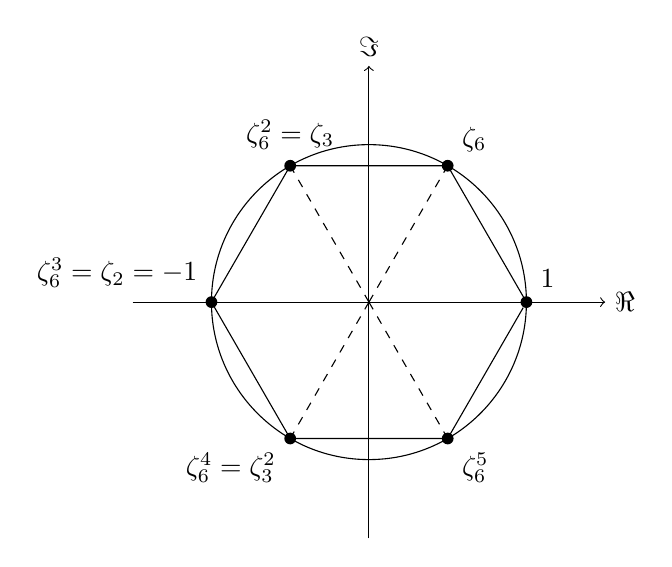
\begin{tikzpicture}[x=2cm,y=2cm]
      \draw (0,0) circle (1);

      \draw (0:1) node[circle,fill,inner sep=1.5pt, label=above right:$1$] (m0) {} --
      (60:1) node[circle,fill,inner sep=1.5pt, label=above right:$\zeta_6$] (m1) {} --
      (120:1) node[circle,fill,inner sep=1.5pt, label=above:{$\zeta_6^2 = \zeta_3$}] (m2) {} --
      (180:1) node[circle,fill,inner sep=1.5pt, label=above left:{$\zeta_6^3 = \zeta_2 = -1$}] (m3) {} --
      (240:1) node[circle,fill,inner sep=1.5pt, label=below left:{$\zeta_6^4 = \zeta_3^2$}] (m4) {} --
      (300:1) node[circle,fill,inner sep=1.5pt, label=below right:{$\zeta_6^5$}] (m5) {} -- (m0);

      \draw[dashed] (0,0) -- (60:1);
      \draw[dashed] (0,0) -- (120:1);
      \draw[dashed] (0,0) -- (240:1);
      \draw[dashed] (0,0) -- (300:1);

      \draw[->] (-1.5,0) -- (+1.5,0) node[right] {$\Re$};
      \draw[->] (0,-1.5) -- (0,+1.5) node[above] {$\Im$};
    \end{tikzpicture}
  \end{center}
  Tenemos
  \[ S_1 = \{ 1 \}, ~ S_2 = \{ \zeta_2 \}, ~ S_3 = \{ \zeta_3, \zeta_3^2 \}, ~ S_6 = \{ \zeta_6, \zeta_6^5 \}. \qedhere \]
\end{ejemplo}

\begin{definicion}
  El $n$-ésimo
  \term{polinomio ciclotómico}\index{polinomio!ciclotómico}\footnote{La palabra
    ``ciclotomia'' significa ``división del círculo'' y se refiere al hecho de
    que las $n$-ésimas raíces de la unidad son vértices de un $n$-ágono regular
    inscrito en el circulo unitario.} es el polinomio mónico que tiene como sus
  raíces las raíces $n$-ésimas primitivas de la
  unidad:\index[notacion]{Fi@$\Phi_n$}
  $$\Phi_n \dfn \prod_{\substack{0 \le a < n \\ \mcd (a,n) = 1}} (X - \zeta_n^k).$$
\end{definicion}

Este polinomio tiene grado $\phi (n)$ y es mónico.

\begin{ejemplo}
  Los primeros polinomios ciclotómicos son
  \begin{align*}
    \Phi_1 & = X - 1,\\
    \Phi_2 & = X + 1,\\
    \Phi_3 & = (X - \zeta_3)\,(X - \zeta_3^2) = X^2 - (\zeta_3 + \zeta_3^2)\,X + \zeta_3^3 = X^2 + X + 1,\\
    \Phi_4 & = (X - \zeta_4)\,(X - \zeta_4^3) = (X - i)\,(X + i) = X^2 + 1. \qedhere
  \end{align*}
\end{ejemplo}

\begin{teorema}
  ~

  \begin{enumerate}
  \item[1)] Para todo primo $p$ se tiene
    $$\Phi_p = \frac{X^p-1}{X-1} = X^{p-1} + X^{p-2} + \cdots + X^2 + X + 1.$$

  \item[2)] Para todo primo $p$ y $k \ge 1$ se tiene
    $$\Phi_{p^k} = \frac{X^{p^k} - 1}{X^{p^{k-1}} - 1} = \Phi_p (X^{p^{k-1}}) = X^{(p-1)\,p^{k-1}} + X^{(p-2)\,p^{k-1}} + \cdots + X^{2p^{k-1}} + X^{p^{k-1}} + 1.$$

  \item[3)] Para todo $n$ se tiene
    $$\prod_{d\mid n} \Phi_d = X^n - 1.$$

  \item[4)] Todos los polinomios $\Phi_n$ tienen coeficientes enteros.
  \end{enumerate}

  \begin{proof}
    Observamos que
    $$\prod_{0 \le a < n} (X - \zeta_n^a) = X^n - 1.$$

    En la parte 1), basta notar que entre las raíces $p$-ésimas, todas son
    primitivas, salvo la raíz trivial $1$, así que
    $$\Phi_p = \prod_{1 \le a < p} (X - \zeta_p^a) = \left.\prod_{0 \le a < p} (X - \zeta_p^a)\right/(X-1) = \frac{X^p-1}{X-1}.$$

    De la misma manera, en 2) notamos que un número $0 \le a < p^k$ tal que
    $\mcd (a, p^k) \ne 1$ es necesariamente divisible por $p$, así que
    las raíces de orden $p^k$ que no son primitivas tienen forma
    $\zeta_{p^k}^{pb} = \zeta_{p^{k-1}}^b$ y son precisamente todas las raíces
    de orden $p^{k-1}$:
    $$\Phi_{p^k} = \prod_{\substack{0 \le a < p^k \\ \mcd (a,p^k) = 1}} (X - \zeta_{p^k}^a) = \left.\prod_{0 \le a < p^k} (X - \zeta_{p^k}^a)\right/\prod_{0 \le b < p^{k-1}} (X - \zeta_{p^{k-1}}^b) = \frac{X^{p^k} - 1}{X^{p^{k-1}}-1}.$$

    En la parte 3), basta notar que
    $$X^n - 1 = \prod_{0\le a < n} (X - \zeta_n^a) = \prod_{d\mid n} \prod_{\substack{0 \le a < n \\ \mcd (a,d) = 1}} (X - \zeta_n^a) = \prod_{d\mid n} \Phi_d,$$
    usando el resultado de \ref{prop:descomposicion-en-raices-primitivas}.

    La parte 4) se demuestra por inducción sobre $n$. Esto es cierto, por
    ejemplo, para $\Phi_1 = X-1$. Luego, si $\Phi_m \in \ZZ [X]$ para todo
    $m < n$, entonces podemos considerar el polinomio
    $$g \dfn \prod_{\substack{d\mid n \\ d\ne n}} \Phi_d \in \ZZ [X].$$
    Este es mónico, siendo un producto de polinomios mónicos. La división con
    resto en el anillo $\ZZ [X]$ nos da
    $$X^n - 1 = q\,g + r, \quad \deg r < \deg g$$
    para algunos $q, r \in \ZZ [X]$, mientras que en el anillo más grande
    $\QQ [X] \supset \ZZ [X]$ se cumple
    $$X^n - 1 = \Phi_n\,g.$$
    Pero para la división con resto en $\QQ [X]$ el cociente y el resto están
    definidos de modo único, así que $r = 0$ y $\Phi_n = q \in \ZZ[X]$.
  \end{proof}
\end{teorema}

\begin{ejemplo}
  Tenemos
  \begin{align*}
    \Phi_4 & = \Phi_2 (X^2) = X^2 + 1,\\
    \Phi_5 & = X^4 + X^3 + X^2 + X + 1,\\
    \Phi_6 & = \frac{X^6 - 1}{\Phi_1\,\Phi_2\,\Phi_3} = \frac{(X^3-1)\,(X^3+1)}{\Phi_1\,\Phi_2\,\Phi_3} = \frac{X^3+1}{\Phi_2} = \frac{X^3+1}{X+1} = X^2 - X + 1,\\
    \Phi_7 & = X^6 + X^5 + X^4 + X^3 + X^2 + X + 1,\\
    \Phi_8 & = \Phi_2 (X^4) = X^4 + 1,\\
    \Phi_9 & = \Phi_3 (X^2) = X^6 + X^3 + 1,\\
    \Phi_{10} & = \frac{X^{10}-1}{\Phi_1\,\Phi_2\,\Phi_5} = \frac{(X^5+1)\,(X^5-1)}{(X^5-1)\,\Phi_2} = \frac{X^5+1}{X+1} = X^4 - X^3 + X^2 - X + 1.
  \end{align*}

  Notamos que
  \begin{gather*}
    \Phi_3 = X^2 + X + 1, \quad \Phi_6 = X^2 - X + 1 = \Phi_3 (-X),\\
    \Phi_5 = X^4 + X^3 + X^2 + X + 1, \quad \Phi_{10} = X^4 - X^3 + X^2 - X + 1 = \Phi_5 (-X).
  \end{gather*}
  Esto no es una coincidencia: en general, $\Phi_{2m} = \Phi_m (-X)$ para todo
  $m > 1$ impar.
\end{ejemplo}

\begin{comentario}
  Aunque revisando los primeros $\Phi_n$ uno puede pensar que los coeficientes
  son siempre iguales a $\pm 1$, para $n = 105 = 3\cdot 5\cdot 7$ en $\Phi_n$
  aparecen por primera vez coeficientes diferentes:

  \begin{multline*}
    \Phi _{105} = X^{48}+X^{47}+X^{46}-X^{43}-X^{42}-\colorbox{shadecolor}{$2X^{41}$} -X^{40}-X^{39}+X^{36}+X^{35}+X^{34}\\
    +X^{33}+X^{32}+X^{31}-X^{28}-X^{26}-X^{24}-X^{22}-X^{20}+X^{17}+X^{16}+X^{15}\\
    +X^{14}+X^{13}+X^{12}-X^{9}-X^{8}-\colorbox{shadecolor}{$2X^{7}$}-X^{6}-X^{5}+X^{2}+X+1.
  \end{multline*}
\end{comentario}

% % % % % % % % % % % % % % % % % % % % % % % % % % % % % %

\section{Polinomios de diversas variables}

La construcción de polinomios puede ser generalizada al
\term{anillo de polinomios con coeficientes en $A$ en $n$ variables
  $X_1,\ldots,X_n$ que se denota por $A [X_1,\ldots,X_n]$}\index{anillo!de
  polinomios!en $n$ variables}\index[notacion]{AX1Xn@$A [X_1,\ldots,X_n]$}.
En este caso los elementos son las expresiones formales de la forma
$$f = \sum_{i_1,\ldots,i_n \ge 0} a_{i_1,\ldots,i_n}\,X_1^{i_1}\cdots X_n^{i_n},$$
donde $a_{i_1,\ldots,i_n} = 0$, salvo un número finito de
$(i_1,\ldots,i_n)$. Las sumas y productos están definidos por
\begin{multline*}
  \left(\sum_{i_1,\ldots,i_n \ge 0} a_{i_1,\ldots,i_n}\,X_1^{i_1}\cdots X_n^{i_n}\right) + \left(\sum_{i_1,\ldots,i_n \ge 0} b_{i_1,\ldots,i_n}\,X_1^{i_1}\cdots X_n^{i_n}\right) \\
  \dfn \sum_{i_1,\ldots,i_n \ge 0} (a_{i_1,\ldots,i_n} + b_{i_1,\ldots,i_n})\,X_1^{i_1}\cdots X_n^{i_n}
\end{multline*}
y
\begin{multline*}
  \left(\sum_{i_1,\ldots,i_n \ge 0} a_{i_1,\ldots,i_n}\,X_1^{i_1}\cdots X_n^{i_n}\right) \cdot \left(\sum_{j_1,\ldots,j_n \ge 0} b_{j_1,\ldots,j_n}\,X_1^{j_1}\cdots X_n^{j_n}\right) \\
  \dfn \sum_{k_1,\ldots,k_n \ge 0} \left(\sum_{\substack{(k_1,\ldots,k_n) = \\ (i_1,\ldots,i_n) + (j_1,\ldots,j_n)}} a_{i_1,\ldots,i_n}\,b_{j_1,\ldots,j_n}\right)\,X_1^{k_1}\cdots X_n^{k_n}.
\end{multline*}

Si quitamos la condición que $a_{i_1,\ldots,i_n} = 0$, salvo un número finito de
$(i_1,\ldots,i_n)$, se obtiene el \term{anillo de las series formales de
  potencias en $n$ variables
  $A [\![X_1,\ldots,X_n]\!]$}\index{anillo!de series formales!en $n$
  variables}\index[notacion]{AX1Xn@$A [[X_1,\ldots,X_n]]$}.

\begin{proposicion}
  \label{prop:A[X1...Xn]-dominio}
  Si $A$ es un dominio, entonces $A [X_1,\ldots,X_n]$ es también un dominio.
\end{proposicion}

Para los polinomios en una variable, lo probamos considerando los términos
mayores: si
$$f = a_m\,X^m + \cdots + a_1\,X + a_0, \quad g = b_n\,X^n + \cdots + b_1\,X + b_0,$$
donde $a_m, b_n \ne 0$, entonces
$$fg = a_m b_n \, X^{m+n} + \cdots + a_0 b_0,$$
donde $a_m b_n \ne 0$. Para los polinomios en diversas variables, ya no está
claro qué termino se puede llamar mayor---considere, por ejemplo, el polinomio
$$f = X^2 Y + X^2 + XY + Y^2 + 1$$
en dos variables $X$ e $Y$.

Como un remedio, podemos considerar el \term{orden lexicográfico} sobre los
monomios $X_1^{i_1}\cdots X_n^{i_n}$: se dice que
$$X_1^{i_1}\cdots X_n^{i_n} \succ_{lex} X_1^{j_1}\cdots X_n^{j_n}$$
si la primera entrada no nula del vector $(i_1-j_1,\ldots,i_n-j_n)$ es
positiva. Esto nos permite definir el término mayor de un polinomio, y cuando
$A$ es un dominio, el término mayor de $fg$ es el producto de los términos
mayores de $f$ y $g$. Dejo los detalles al lector.

Otra opción (pero esencialmente equivalente) es aislar una variable y expresar
cada polinomio como una suma $\sum_i f_i \, X_n^i$, donde
$f_i \in A [X_1,\ldots,X_{n-1}]$. Por ejemplo, para el polinomio de arriba
$$f = Y^2 + (X^2 + X)\,Y + (X^2 + 1).$$

\begin{proof}[Demostración de \ref{prop:A[X1...Xn]-dominio}]
  Para $n=1$ esto ya fue probado arriba. Procedamos por inducción sobre
  $n$. Sean
  $$f = \sum_{i_1,\ldots,i_n} a_{i_1,\ldots,i_n}\,X_1^{i_1}\cdots X_n^{i_n}, \quad g = \sum_{j_1,\ldots,j_n} b_{j_1,\ldots,j_n}\,X_1^{j_1}\cdots X_n^{j_n}$$
  dos polinomios no nulos. Podemos escribirlos como
  $$f = \sum_{0 \le i \le p} f_i (X_1,\ldots,X_{n-1})\,X_n^i, \quad g = \sum_{0 \le j \le q} g_j (X_1,\ldots,X_{n-1})\,X_n^j$$
  donde $f_i$, $g_j$ son polinomios en variables $X_1,\ldots,X_{n-1}$ y
  $f_p, g_q \ne 0$. Luego, el coeficiente mayor de $fg$ es $f_p g_q$ que no es
  nulo por la hipótesis de inducción.
\end{proof}

\iffalse
Notamos que si
$$X_1^{i_1}\cdots X_n^{i_n} \succ_{lex} X_1^{j_1}\cdots X_n^{j_n},$$
entonces
\begin{equation}
  \label{eqn:lex-orden-monomial}
  (X_1^{i_1}\cdots X_n^{i_n})\cdot (X_1^{k_1}\cdots X_n^{k_n}) \succ_{lex} (X_1^{j_1}\cdots X_n^{j_n})\cdot (X_1^{k_1}\cdots X_n^{k_n}).
\end{equation}
Para un polinomio no nulo
$$f = \sum_{i_1,\ldots,i_n} a_{i_1,\ldots,i_n}\,X_1^{i_1}\cdots X_n^{i_n} \in A [X_1,\ldots,X_n],$$
denotemos por
$$TM (f) \dfn \max \{ a_{i_1,\ldots,i_n}\,X_1^{i_1}\cdots X_n^{i_n} \mid a_{i_1,\ldots,i_n} \ne 0 \}$$
el \term{término mayor} respecto al orden lexicográfico.

\begin{proof}[Demostración de \ref{prop:A[X1...Xn]-dominio}]
  De nuevo, por inducción sobre el número de variables, tenemos
  $$\left(\sum_i f_i\,X^i\right)\,\left(\sum_j g_j\,X^j\right) = \sum_k \left(\sum_{i+j=k} f_i g_j\right)\,X_n^k = 1,$$
  de donde $f_0 g_0 = 1$ y $f_i g_j = 0$ para $i > 0$ o $j > 0$. Entonces,
  $f_i = g_j = 0$ para $i > 0$ o $j > 0$, mientras que $f_0$ y $g_0$ deben ser
  constantes por la hipótesis de inducción.
\end{proof}
\fi

\begin{proposicion}
  \label{prop:A[X1...Xn]-elementos-invertibles}
  Si $A$ es un dominio, entonces los elementos invertibles en
  $A [X_1,\ldots,X_n]$ son los polinomios constantes invertibles en $A$.

  \begin{proof}
    Por inducción sobre el número de variables se demuestra que el término
    constante debe ser invertible:
    $$fg = \sum_{k\ge 0} \left(\sum_{i+j = k} f_i g_j\right)\,X_n^k = 1,$$
    y luego,
    $$f_0 g_0 = 1.$$
    Para ver que no puede haber términos no constantes, hay que usar el hecho de
    que si $A$ es un dominio, entonces el término mayor de $fg$ es el producto
    de los términos mayores.
  \end{proof}
\end{proposicion}

Los polinomios en diversas variables no funcionan de la misma manera que
los polinomios en una variable. En particular, en $k [X_1,\ldots,X_n]$ no existe
la división con resto que hemos ocupado en este capítulo para probar varios
resultados sobre $k [X]$. La teoría de ecuaciones polinomiales en diversas
variables es también mucho más sofisticada. El lector interesado puede consultar
el libro introductorio \cite{Cox-Little-OShea-intro}.
